% ------------------------------------------------------------------------------
% Slide 0: Portada
% ------------------------------------------------------------------------------
\begin{frame}[plain]
    \titlepage
\end{frame}

% ------------------------------------------------------------------------------
% Slide 1: Física del Tracto Vocal: El Modelo de Dos Tubos
% ------------------------------------------------------------------------------
\begin{frame}{Física del Tracto Vocal: El Modelo de Dos Tubos}
    \begin{columns}[c]
        \begin{column}{0.51\textwidth}
            \scriptsize
            \begin{block}{Resonancia y Filtrado Acústico}
                Las vocales se producen mediante el filtrado acústico del tracto vocal sobre el tren de pulsos glóticos, determinando las formantes principales ($F_1$ y $F_2$).
            \end{block}
            \vspace{0.03cm}
            \begin{block}{Aproximación de Dos Tubos Acoplados}
                A primer orden, el tracto se comporta como un \textbf{resonador de Helmholtz doble}: las frecuencias propias dependen del volumen de las cavidades y del área de constricción entre ellas.
            \end{block}
            \vspace{0.03cm}
            \begin{alertblock}{Tres Actuadores Mecánicos Principales}
                \begin{itemize}\setlength{\itemsep}{1pt}\setlength{\parskip}{0pt}
                    \item \textbf{Bajar la mandíbula:} abrir la boca con el digástrico, agranda la cavidad bucal y sube $F_1$.
                    \item \textbf{Estirar los labios adelante:} hacer trompita con el orbicular, alarga el tubo acústico y baja $F_2$.
                    \item \textbf{Mover la lengua:} la posición de la lengua adentro cambia el volumen de cada tubo y fija $F_2$.
                \end{itemize}
            \end{alertblock}
        \end{column}
        \begin{column}{0.47\textwidth}
            \centering
            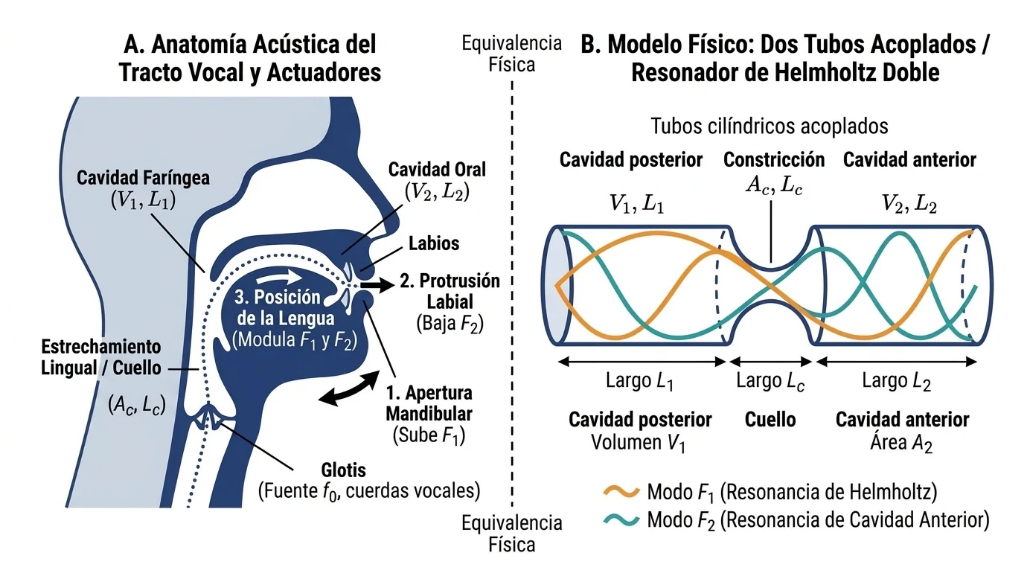
\includegraphics[width=\linewidth,height=0.72\textheight,keepaspectratio]{figuras/esquema_fisica_dos_tubos_helmholtz.png}
        \end{column}
    \end{columns}
\end{frame}
